%% LyX 1.6.7 created this file.  For more info, see http://www.lyx.org/.
%% Do not edit unless you really know what you are doing.
\documentclass[english]{article}
\usepackage[T1]{fontenc}
\usepackage[latin9]{inputenc}
\usepackage{amsmath}
\usepackage{graphicx}
\usepackage{amssymb}
\usepackage{babel}

\begin{document}

\title{YCP Robot}


\author{Tori Bare, Cory Boyle, Jason Cluck, Drew Wicke}


\date{November 21 2011}
\maketitle
\begin{abstract}
The project that was completed in fulfillment of the CS481 requirement
was the design and implementation of software that made a robot both
mobile and autonomous. The group members for this project are Tori
Bare, Cory Boyle, Jason Cluck and Drew Wicke. Using the Robot Operating
System (ROS), algorithms were developed for obstacle avoidance, 3D
navigation, and gesture recognition. Additionally, a simulator was
created in OpenGL that was used as a testbed for these algorithms.
\end{abstract}

\part*{Introduction}

One of the goals of the Robot Operating System (ROS) is to provide
roboticists a software platform for specific robots. <insert quote
on how this improves research> <insert what robots are implemented
in ros already> This paper addresses the construction of a new ROS
package that controls the X80SVP robot. The package, which already
implements obstacle avoidance and wandering behavior, provides low
level drivers up to a robust development framework that can be extended. 

Another goal of the ROS community is to provide simulation software
to test the robot. For example, the player project consists of Player,
a robot interface, Stage, a two-dimensional robot simulator, and Gazebo,
a three-dimensional robot simulator. The paper describes a new simulator
for ROS that can be extended and provides a kinect sensor. 

The paper is organized as follows: the first part provides a background
detailing the devices, algorithms and libraries that were used; the
second part discusses the design of the system following with implementation
details; finally, it concludes with an overview of future work.


\part*{Background}

Various devices, technologies and algorithms were used to create an
autonomous robot. The robot that was used was an X80SVP. A Beagleboard
hosted the software and acted as a bridge to the robot while the Robot
Operating System provided a framework for the software. Braitenburg
aggression behavior was used to provide obstacle avoidance and a Kinect
was used to provide vision. Lastly, OpenGL was used to provide 3D
graphics for the simulator.


\section*{Devices}

The X80SVP Robot has a max speed of 75 cm/s, weighs 3.5 kg, has a
max payload of 15 kg, and has a three hour battery life. The robot
also has IR and ultrasonic range sensors, as well as pyro-electric
human motion sensors.

%
\begin{figure}
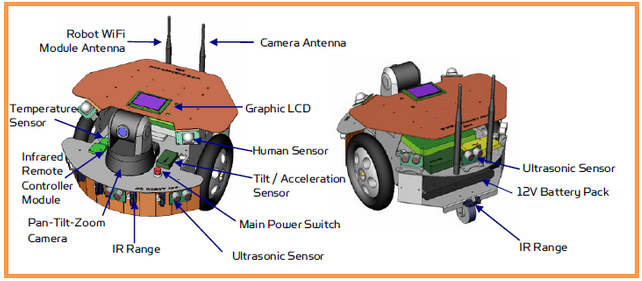
\includegraphics[scale=0.75]{images/X80SVPRobot}

\caption{X80SVP Robot}



\end{figure}


The Beagleboard XM was chosen as the computer for the X80SVP. Some
of the major advantages to this is that the Beagleboard has many peripheral
options, a 1 GHz CPU, a DSP, and it is very popular in the open source/ROS
communities. The initial plan accounted for the DSP being able to
process the Kinect vision data while the CPU handled the overhead
associated with ROS. The major components on the board are shown below
in Figure (2).

%
\begin{figure}
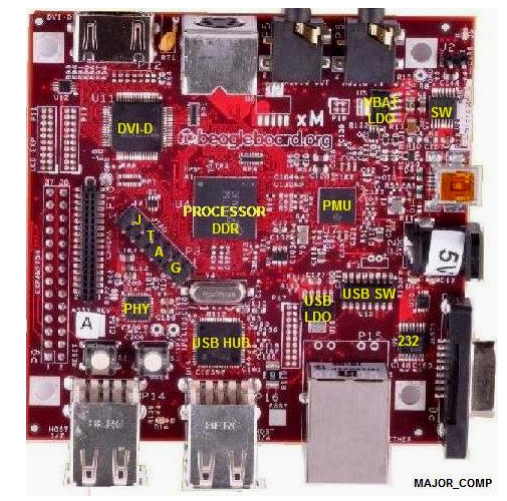
\includegraphics[scale=0.4]{images/beagleboardMajorComps}

\caption{Beagleboard's Main Components}



\end{figure}


A Kinect was used to generate maps of the robot's surroundings and
to allow the robot to navigate intelligently through his environment.
One of the main concerns with using the Kinect was the processing
power that it would require. The Kinect produces a message that is
roughly 10 MB at a rate of 30 frames per second, this equates to the
Kinect sending about 300 MB of data each second. At first, it was
expected that the DSP on the Beagleboard would have been able to handle
the Kinect\textquoteright{}s processing; however, due to the overhead
of ROS, the processing will most likely have to be offloaded to a
netbook. 


\section*{Technologies}

ROS is a framework that facilitates the construction and execution
of applications for robots. There are implementations of ROS in C++,
Python, Lisp, and Java. ROS executables are called nodes. ROS provides
a master node that oversees running nodes and a parameter server,
it also acts as the matchmaker for nodes and topics. ROS nodes communicate
over topics or services using ROS methods. Nodes publish messages
on topics which other nodes can subscribe to in order to receive the
information. The message's fields are described in a data file using
the yaml language which ROS converts into a file that the targeted
language can use, such as a header file in C++.

ROS also provides a hierarchy to group common elements. Nodes that
perform common functions are grouped into a package. Packages that
share a common purpose are grouped into stacks. Therefore, ROS's goal
is to build a complex system out of simple, single-purpose parts.

The rosjava stack is an implementation of ROS in Java; therefore,
rosjava nodes work with the rest of the nodes in ROS. In order for
rosjava nodes to communicate, ROS messages are converted to classes
and made into jar files; this allows for easy integration of message
data types into rosjava nodes.


\section*{Obstacle Avoidance Algorithm}

There are two ways to implement obstacle avoidance. One implementation
is motor fusion, which uses a direct correlation between sensor readings
and motor velocities. The second implementation, sensor fusion, uses
the sensor data to reconstruct the surroundings to produce motor commands.
For the X80SVP robot, obstacle avoidance was accomplished by a motor
fusion algorithm utilizing Braitenburg's aggression behavior. Braitenburg
behaviors are a form of synthetic psychology described in Valentino
Braitenberg\textquoteright{}s book. These behaviors were thought experiments
into how different emotions, such as fear, aggression, and love, can
provoke movement based on sensor stimulation. Aggression behavior
is caused by pairing the sensors and motors on opposite sides through
a non-decreasing function.

To implement aggression behavior for obstacle avoidance, modifications
to use a centered sensor were made to the algorithm presented in \cite{ran2005obsavothrbraaggbehmotfus}.
The algorithm computes both the linear and angular velocity for the
robot given the normalized sensor readings as shown in equations \ref{eq:translationalSpeed}
and \ref{eq:rotationalSpeed}. Accounting for the center sensor separately
allows the robot to avoid deadlock while in symmetric corners. The
value of the sensor increases as an obstacle gets farther away and
as the velocity becomes greater in that direction, providing a smooth
wandering movement that effectively avoids obstacles.

\begin{equation}
\alpha_{S}(t_{k})=\sum_{i\in L\cup R}w_{i}^{\alpha_{S}}\hat{r}_{i}^{S}(t_{k})\label{eq:translationalSpeed}\end{equation}


\begin{equation}
\beta_{S}(t_{k})=\sum_{i\in R}w_{i}^{\beta_{S}}\mathfrak{D}(\theta'_{i})\hat{r}_{i}^{S}(t_{k})-\sum_{i\in L}w_{i}^{\beta_{S}}\mathfrak{D}(\theta'_{i})\hat{r}_{i}^{S}(t_{k})\label{eq:rotationalSpeed}\end{equation}


$\alpha_{S}$ and $\beta_{S}$ are the normalized translational and
rotational speeds in the range {[}0,1{]} and {[}-1,1{]} respectivley.
$w_{i}^{\alpha_{S}}$ and $w_{i}^{\beta_{S}}$ are constant weights
corresponding to the $i^{th}$sensor defined in equations \ref{eq:translationalWeight}
and \ref{eq:rotationalWeight}. $\hat{r}_{i}^{S}(t_{k})$ is the current
normalized filtered range value of the $i^{th}$ sensor. $\mathfrak{D}(\theta'_{i})=90-|\theta_{i}|$
the angular distance. Where $\theta_{i}$ is angle from the x-axis
to the sensor assuming the x-axis lies on the axle and y-axis divides
the robot in half.

\begin{equation}
\mathit{w}_{i}^{\alpha_{S}}=k_{i}^{\alpha}e^{-\frac{\mathfrak{D}(\theta'_{i})^{2}}{2\sigma_{\alpha}^{2}}}\label{eq:translationalWeight}\end{equation}


\begin{equation}
\mathit{w}_{i}^{\beta_{S}}=k_{i}^{\beta}e^{-\frac{\mathfrak{D}(\theta'_{i})^{2}}{2\sigma_{\beta}^{2}}}\label{eq:rotationalWeight}\end{equation}


$k_{i}^{\alpha}$ and $k_{i}^{\beta}$ are normalizing constants so
that the speeds are normalized. $\sigma_{\alpha}^{2}$ and $\sigma_{\beta}^{2}$
are the variance chosen here to be 1400 and 350 respectively. 


\section*{Libraries}

The simulator uses a number of libraries to make the OpenGL API more
manageable. FreeGLUT is used to provide the basic windowing functions
for the GL application. GLU provides utility functions for computing
projection matrices, used to create the perspective camera views.
SOIL is used to provide texture-loading capabilities. The simulator
also interfaces directly with the Xorg APIs for some functions in
handling mouse and full-screen controls. A custom loader was written
to load DirectX format mesh files exported by Blender. This allows
environments as well as movable obstacles of completely arbitrary
design and complexity to be modelled quickly.


\part*{Design}

The design model favors modularity and simplicity to create a complex
system. The goal was to follow the subsumption control architecture
to create a robust and fault tolerant system. By following the model
view controller design pattern, the implementation is extensible.
The model is based on the ROS parameter server in which the model
of the robot and communication layout is stored. The view is the world
or the virtual world as created by the simulator. The controller classes
act to move the robot, changing the robot\textquoteright{}s view. 

The design is centered around the Converter and the RobotActor classes.
Converter and RobotActor are interchangeable bridges between the view
and the control, they publish the sensor data and send commands to
actuate the robot\textquoteright{}s motors. The SensorListener class
subscribes to the sensor messages published by a bridge class and
publishes converted sensor data in the ROS standard Range message
type. The SensorFilter classes filter the sensor data so that the
data is more useful and the BraitenburgAvoid class uses the filtered
sensor data to publish a MotorCommand message based on the Braitenburg
aggression behavior algorithm. The ObstacleAvoidance node publishes
a linear combination of the MotorCommand sent by the infrared and
ultrasonic based on BraitenburgAvoid nodes. Finally, the MotorController
acts as both an arbiter of motor commands and as a gateway back to
the bridge nodes.


\part*{Implementation}

The implementation of the design was completed in both C++ and Java.
C++ was used for the simulator and the serial communication between
the robot and Beagleboard while Java was used to implement the rest
of the design.

The serial library used the PMS5005 protocol which allows any processor,
DSP, or PC to control the robot through the Universal Asynchronous
Receiver/Transmitter (UART) communication interface. The basic packet
outline, shown in Figure N, handles both the sensor and motor data
transmission. The library that implements this interacts with ROS
by subscribing to motor controls and publishing sensor data. Using
this packet structure, a large amount of information can be processed
every tick.

%
\begin{figure}
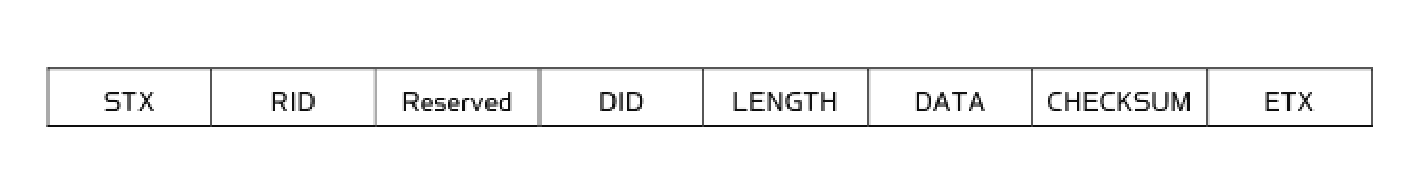
\includegraphics[scale=0.5]{images/packet}

\caption{Packet format for serial library}

\end{figure}


Once the serial library was implemented on a desktop system, the next
step was to achieve this functionality on the Beagleboard. The Beagleboard
was loaded with Ubuntu 11.10 since this OS would work best with ROS.
Some of the configuration scripts for ROS requires Internet access
so a wireless internet connection was also part of the Beagleboard
setup. 

The obstacle avoidance algorithm produces linear and angular velocity
values, but the robot requires left and right wheel velocities. Using
the differential drive kinematics equations \ref{eq:LeftVelocity}
and \ref{eq:RightVelocity}, the conversion is possible.

\begin{equation}
V_{L}=\frac{2\alpha_{S}(t_{k})+d\beta_{S}(t_{k})}{2}\label{eq:LeftVelocity}\end{equation}


\begin{equation}
V_{R}=V_{L}-d\beta_{S}(t_{k})\label{eq:RightVelocity}\end{equation}


Ultrasonic sensors were used to provide obstacle avoidance, however
the sensors can overestimate the distance to a flat wall due to specular
reflection. These readings can be improved by applying an incremental
filter (Equation \ref{eq:USFilter}) as described in \cite{ran2005obsavothrbraaggbehmotfus}.
The filter works by acting as a short term memory to ensure that a
current reading of free space is correct based on the previous range. 

\begin{equation}
\tilde{r_{i}}(t_{k})=\begin{cases}
r_{i}^{s}(t_{k}) & \textrm{if }r_{i}^{s}(t_{k})<r_{nr}^{s}\\
Min\{\tilde{r_{i}}(t_{k-1})+r_{\triangle},r_{nr}^{s} & \textrm{if }r_{i}^{s}(t_{k})=r_{nr}^{s}\end{cases}\label{eq:USFilter}\end{equation}


$r_{nr}^{s}$is the max range of the sensor, $r_{i}^{s}(t_{k})$ is
the current range measurement, $\tilde{r_{i}}(t_{k})$ is the current
filtered range value and $\tilde{r_{i}}(t_{k-1})$ is the previous
filtered value.

One issue of using rosjava was the overhead of creating new nodes,
since each new node started a new JVM process. After implementing
the design of the rosjava nodes, rosjava released documentation detailing
how using a NodeRunner object can start the nodes as threads rather
than as new processes. This significantly reduced the memory overhead
and launch time of the rosjava nodes.


\part*{Future Work}

The system could be extended by adding turtlebots to create a multi-agent
system. Capture the flag could be a way to explore algorithms involved
in multi-agent systems. However, due to the limited processing power
of the BeagleBoard there would be considerable challenges implementing
efficient navigation, SLAM and learning algorithms. One solution would
be to use a remote computer to perform these features. 

Another way the system could be extended is by using the kinect for
facial and object recognition. This would allow for high level behavior
and learning rather than the current reactive based system. However,
processing capabilities of an on-board computer may be overwhelmed. 

A future system could also utilize rosjava\textquoteright{}s ability
to operate on android to provide a user with the ability to teleoperate
the robot or provide the robot access to the cloud.

\bibliographystyle{plain}
\nocite{*}
\bibliography{bibliography}

\end{document}
